\documentclass[english]{article}\usepackage[]{graphicx}\usepackage[]{color}
%% maxwidth is the original width if it is less than linewidth
%% otherwise use linewidth (to make sure the graphics do not exceed the margin)
\makeatletter
\def\maxwidth{ %
  \ifdim\Gin@nat@width>\linewidth
    \linewidth
  \else
    \Gin@nat@width
  \fi
}
\makeatother

\definecolor{fgcolor}{rgb}{0.345, 0.345, 0.345}
\newcommand{\hlnum}[1]{\textcolor[rgb]{0.686,0.059,0.569}{#1}}%
\newcommand{\hlstr}[1]{\textcolor[rgb]{0.192,0.494,0.8}{#1}}%
\newcommand{\hlcom}[1]{\textcolor[rgb]{0.678,0.584,0.686}{\textit{#1}}}%
\newcommand{\hlopt}[1]{\textcolor[rgb]{0,0,0}{#1}}%
\newcommand{\hlstd}[1]{\textcolor[rgb]{0.345,0.345,0.345}{#1}}%
\newcommand{\hlkwa}[1]{\textcolor[rgb]{0.161,0.373,0.58}{\textbf{#1}}}%
\newcommand{\hlkwb}[1]{\textcolor[rgb]{0.69,0.353,0.396}{#1}}%
\newcommand{\hlkwc}[1]{\textcolor[rgb]{0.333,0.667,0.333}{#1}}%
\newcommand{\hlkwd}[1]{\textcolor[rgb]{0.737,0.353,0.396}{\textbf{#1}}}%
\let\hlipl\hlkwb

\usepackage{framed}
\makeatletter
\newenvironment{kframe}{%
 \def\at@end@of@kframe{}%
 \ifinner\ifhmode%
  \def\at@end@of@kframe{\end{minipage}}%
  \begin{minipage}{\columnwidth}%
 \fi\fi%
 \def\FrameCommand##1{\hskip\@totalleftmargin \hskip-\fboxsep
 \colorbox{shadecolor}{##1}\hskip-\fboxsep
     % There is no \\@totalrightmargin, so:
     \hskip-\linewidth \hskip-\@totalleftmargin \hskip\columnwidth}%
 \MakeFramed {\advance\hsize-\width
   \@totalleftmargin\z@ \linewidth\hsize
   \@setminipage}}%
 {\par\unskip\endMakeFramed%
 \at@end@of@kframe}
\makeatother

\definecolor{shadecolor}{rgb}{.97, .97, .97}
\definecolor{messagecolor}{rgb}{0, 0, 0}
\definecolor{warningcolor}{rgb}{1, 0, 1}
\definecolor{errorcolor}{rgb}{1, 0, 0}
\newenvironment{knitrout}{}{} % an empty environment to be redefined in TeX

\usepackage{alltt}
\usepackage{hyperref}
\usepackage{geometry}
\geometry{verbose,tmargin=1in,bmargin=1in,lmargin=1in,rmargin=1in}
\usepackage{fancyhdr}
\pagestyle{fancy}
\setlength{\parskip}{\smallskipamount}
\setlength{\parindent}{0pt}
\usepackage{amsthm}
\usepackage{amsmath}
\IfFileExists{upquote.sty}{\usepackage{upquote}}{}
\begin{document}

\title{Lab 1 - Redwood Data, Stat 215A, Fall 2017}

\author{Alexander J. Brandt}

\maketitle





\section{Introduction}

In this report we will investigate the data cleaning and analysis methodologies undertaken by Tolle et. al. in their study of climate dynamics as experienced by a California coastal redwood.\\\\
The data is recieved without any explanation as to the variables or their collection
methodologies except for those that are specified in the paper, and
imply questions surrounding their collection and interpretation.  The redwood sensors (or ``motes'')
originally were intended to pass data to a central computer via wireless network.  It was
later determined that the wireless data collection system was faulty or defective, and
so as a result, digital logs stored on flash memory chips within the sensors themselves 
proved to be the most reliable source of data according to the collaborators.  Both the 
networked collected and log collected data sets were made avalible.

\section{The Data}

\subsection{Data Collection}
The sensors were built with the following sensors, though the significant ones are bolded.
\begin{itemize}
\item \textbf{Time -- each sensor tracks the time of each measurement taken.  It accomplishes this by briefly turning on once every 5 minutes to both ensure periodicity and conserve battery.}
\item \textbf{Temperature -- a standard electronic thermometer, probably based on resistors with a known thermal drift}
\item \textbf{Humidity -- a measure of the amount of water vapor in the local atmosphere surrounding the mote.  Given as a percent humidity rather than mmHg or atm.}
\item Barometric pressure -- A barometer measuring atmospheric pressure.  Not used to do sensitivity issues.
\item \textbf{Light Levels (Photosynthetic Active Radiation) -- a photometer measuring photosynthetic active radiation in PPFD (photosynthetic photon flux density).  Values were taken at the top and bottom of the mote.}
\item Light Levels (TSR) -- a photometer measuring total active radiation in a broader spectrum.  Not used do to sensitivity issues.
\item \textbf{Voltage -- the remaining voltage in the mote's battery.}
\item \textbf{Node ID -- the numerical identity of the node that has collected the data (important for associating physical properties later).}
\end{itemize}

\subsection{Data Cleaning}

Since the redwood data set was collected from two sources (the network and the backup data logs stored in the sensors), the concatenated data set might be redundant. We attempted to check the consistency of the
two constituient data sets before blindly proceeding with the log based data set as the authors suggested.

\begin{enumerate}
\item The authors of the paper suggest that the log data set will be more complete 
and therefore useful than the network data set.  We inner join the two as data frames 
and check to see that their values correlated correctly.  All measurements
but voltage are well correlated.  Voltage comparisons between the two are problematic.
This will flag voltage as an important variable to consider in the data cleaning.

\begin{center}
\begin{tabular}{ c || c }
 Measurement & Log/Net Correlation \\ \hline
 Humidity & 1 \\
 Temperature & 1 \\
 Incoming Light & 1 \\
 Outgoing Light & 0.9999496 \\
 Voltage & -0.9961888 \\

\end{tabular}
\end{center}

Because the log data set is more complete, and the mutual entries appear to be mostly consistent,
we proceed with using the log data set.

\item We notice a bulk of the voltage exist at exactly 0.580567 V (26040 entries), which is probably a default value set by the firmware.  With such a large volume of the 
observations corresponding to this value, we leave them in for later investigation (this 
will form the basis of our first observation).
\item We notice the time in the log data set is systematically wrong (it is a constant value, 
probably from when the researchers downloaded the data from the motes).  We perform a merger
with a table that corresponds between ``epoch'' (the serial counting of 5 minute intervals),
and the local time in UTC.  We then convert the UTC to Pacific Time so we can have an 
intuitive understanding of daylight.
\item We remove extreme outlines from the data set for temperature and humidity.  For
our criteria, we allow values slightly outside physical reality (slightly less than 0\%
and slightly more than 100\%, since this is within the error of the instrument).
But we remove humidities of less than -100\% or more than 200\%.
We also remove temperatures of less than -10 C (since there is a large, discontinuous cluster at 
-38.4 C, and this value is simply nonsensical given the local climate).
\item Finally, we selection just the nodes that correspond to the interior tree (there are two 
trees in the data set), since the paper only seemed to analyze the interior tree, as well as nodes
that fall within the 0 - 200 node id range (there was one node with an invalid ID).
\end{enumerate}

\begin{knitrout}
\definecolor{shadecolor}{rgb}{0.969, 0.969, 0.969}\color{fgcolor}

{\centering 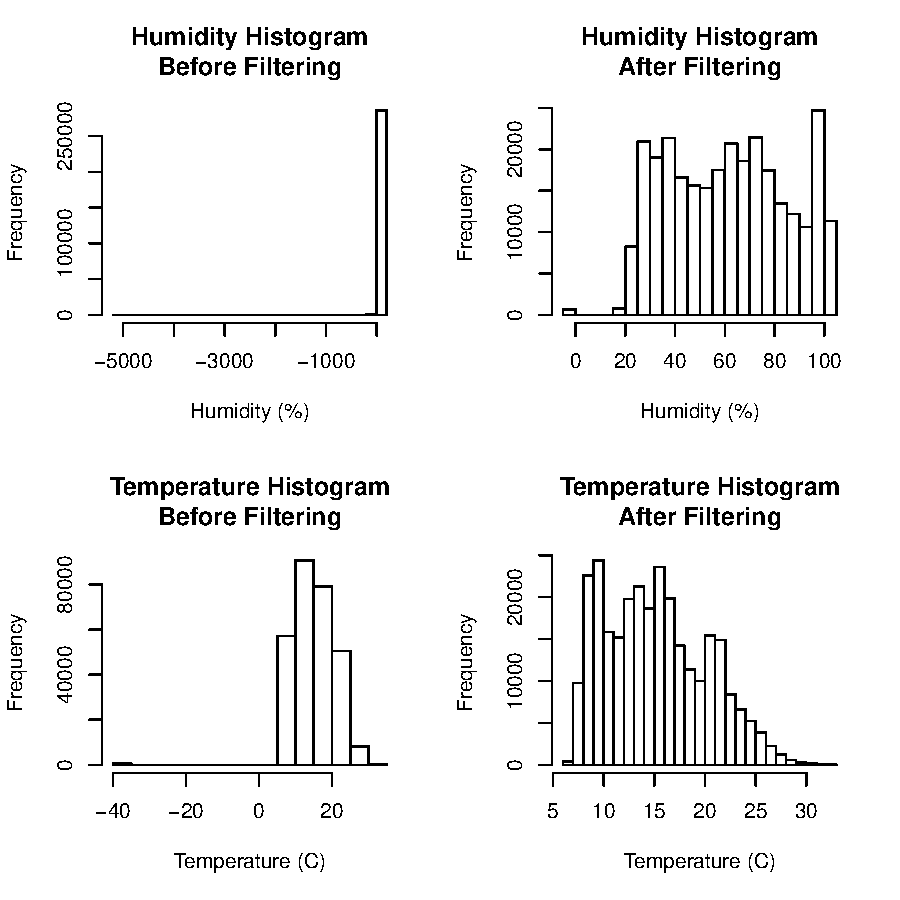
\includegraphics[width=\maxwidth]{figure/load-data-1} 

}



\end{knitrout}

\subsection{Data Exploration}

\section{Graphical Critique}

\subsection{Figure 3}

This figure has several issues.  I found the first set of histograms to be relatively
useful, especially with respect to troubleshooting my own analyses.\\\\
The temperature and relative humidity are reasonably cogent.  The incident PAR and 
reflected PAR graphs though have very little value, given that they show
what seems to be a constant daily trend.  If there is any other trend it is
incredibly difficult to ascertain.\\\\
Given the distributions shown in part (d) of this figure, these seem fairly redundant.
The boundary between the upper quartile and the outliers are very faint, almost to the
point of illegibility in the case of the incident PAR and reflected PAR.  It may have
been better to remove these figures in order to make part (d) larger.  Or maybe represented
as a heat map with color corresponding to probability density.

\subsection{Figure 4}

For the first two time trajectory graphs, I think the colored lines don't
add very much to the comprehension of these graphs.  Probably better would be
an average trajectory with a standard deviation, and min/max lines.  This would
allow for the appreciation of the variance of the measurements at any given point
in time, while making the figure feel less cluttered.  The summary figures seem fine,
except for the Reflected PAR graph which is very hard to read and whose mostly empty
plot seems a waste of space.  There coloring of the motes points (blue/pink) is never explained.

\section{Findings}

To restrict our analysis we pick April 30th (one day before the authors' chosen day)
in order to select a day early in the experiment, where a large number of intact/productive
mote recordings can be found, and to show some different conclusions from those drawn
by figure 3 and figure 4.

\subsection{First finding}

When we cleaned our data set we assumed that the large spike in voltage
at about .58 corresponded to a systematic failure of the voltage analysis
but we will now rigorously investigate that claim.  Let us take two of the most
 temperature and humidity, and analyze them in a pairwise graph
colored by the voltage of their relative mote.  Here we see that the measurements
at low voltages are well blended with the measurements at the higher voltages.
Indeed, we see no relative difference in the patterns, which we have plotted at 
a low alpha value so as not to obscure the general trend.  This graph can add
support to our revised data cleaning practice of including measurements from 
sensors that register with a voltage of lower than 2 V (or even 1 V) to add a large number
of humidity and temperature readings.  But what about for the other units were are interested in?
How would low voltage affect light flux at the top and bottom of the mote?


\begin{knitrout}
\definecolor{shadecolor}{rgb}{0.969, 0.969, 0.969}\color{fgcolor}

{\centering 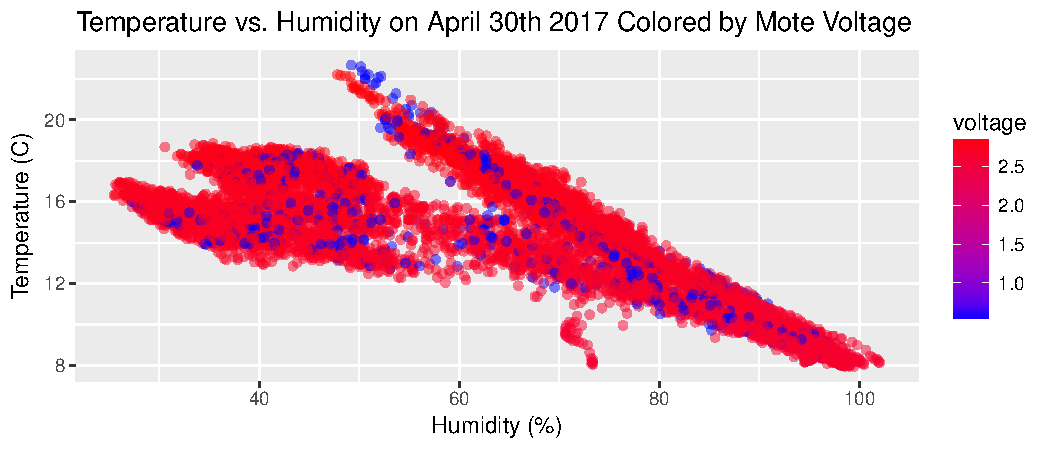
\includegraphics[width=\maxwidth]{figure/q1p1-1} 

}



\end{knitrout}

As opposed to the humidity and temperature readings, the mote voltage does seem to
be prohibitive for understanding photometer readings.  The low voltage motes are much
less senstive to PAR sunlight than the adequatley charged nodes.  We could hypothesize that 
this could be because the photometer elements in the motes are
more power intensive than the humidity or temperature sensor.  Regardless, we should
be skeptical of our light readings from motes with low battery voltage.

\begin{knitrout}
\definecolor{shadecolor}{rgb}{0.969, 0.969, 0.969}\color{fgcolor}

{\centering 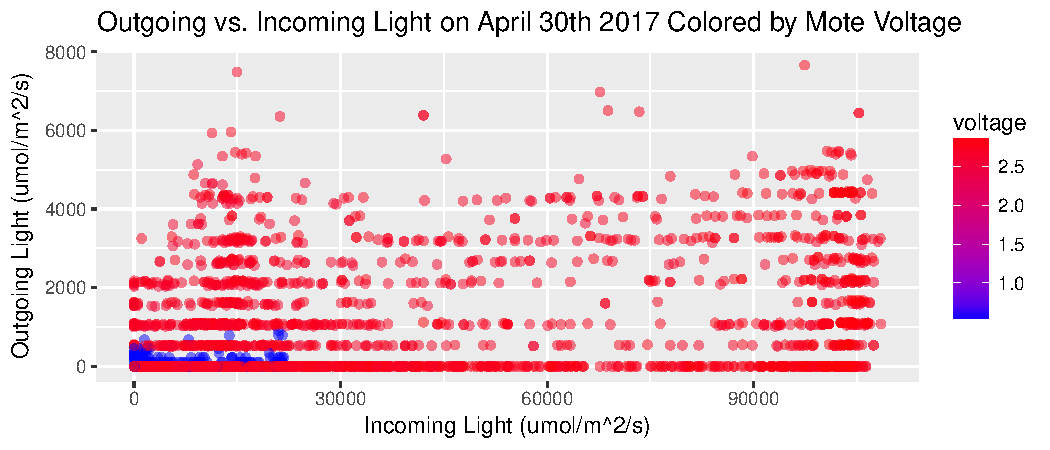
\includegraphics[width=\maxwidth]{figure/q1p2-1} 

}



\end{knitrout}

\subsection{Second finding}

Again, given that we are working with the data without any correspondence
with the authors of the paper, we hope to recapitulate basic physical principles 
as a check on our data clarity and cleaning principles.  Here we examine basic meteorological relationships on April 30th.\\\\
Basic chemical and physical principles tell us that warmer air can bind more
water than cooler air (this is one reason for the ''haze'' seen in cities on muggy days).
So, assuming a constant volume of water, an increase in temperature usually
corresponds to a decrease in relative humidity.  This relationship is recapitulated
in this graph (and has a not unreasonable correlation coefficient of 
-0.8849986).\\

\begin{knitrout}
\definecolor{shadecolor}{rgb}{0.969, 0.969, 0.969}\color{fgcolor}

{\centering 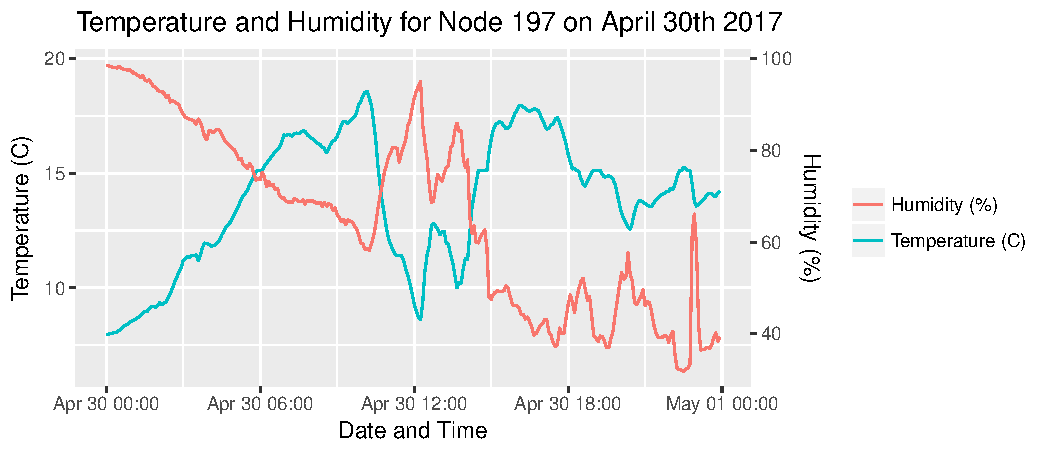
\includegraphics[width=\maxwidth]{figure/q2-1} 

}



\end{knitrout}

So when the authors seem to suggest that on May 1st the tree experienced a microclimate that
didn't obey conventional wisdom around humididty/temperature relationships, I became suspicious and re-plotted it with my expanded
data set that included the lower voltage motes (given that I suspect their climate data is
fine to use for the analysis for reasons stated above).  Indeed, the conventional relationship
between humidity and temperature as a function of time seems to be re-established.  I believe
their conclusions were potentially faulty because they overzealously cleaned their data.\\\\
I would need to check for the trajectories in aggregate, rather than just this one node, to say
definitively if their conclusions were faulty, but in the interests of looking at different types
than just the ones presented in this paper I did not do so.

\begin{knitrout}
\definecolor{shadecolor}{rgb}{0.969, 0.969, 0.969}\color{fgcolor}

{\centering 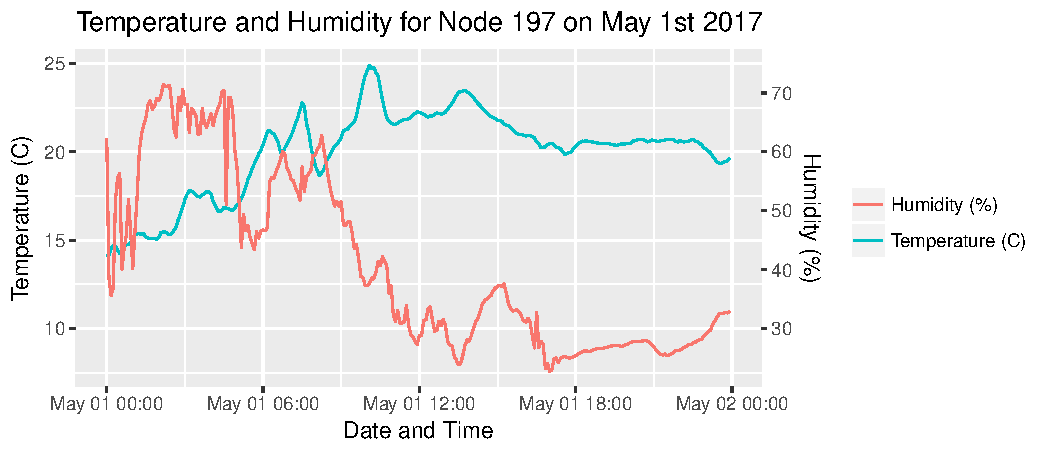
\includegraphics[width=\maxwidth]{figure/q2_2-1} 

}



\end{knitrout}

As an aside, with these two trajectories of information, we could calculate the dew point at
each sensor for the day, if we cared to.

\subsection{Third finding}

Another consistency we would like to investigate is the relationship between temperature and sun exposure.
Redwoods are famously large/tall trees.  In order to isolate minimum shading from the leaves and branches, 
we will investigate the relationship between node height and sun exposure.  We first attempt to check our
assumption that tree node height corresponds with average daily sun exposure (which we will determine by
looking at values from the top photometer of the mote).  We will need to subselect for voltages above a 
certain threshold (here, 2 V).  This filtering only removes 3 nodes from the data set.  A screenshot from the
3D plot is shown below, but the interactive graph can be found in this directory (filename: graph3.html).\\\\
By moving around the interaction you can visualize a coherent trend between the three variables.
Cross sections of the graph are also shown below.

\begin{center}
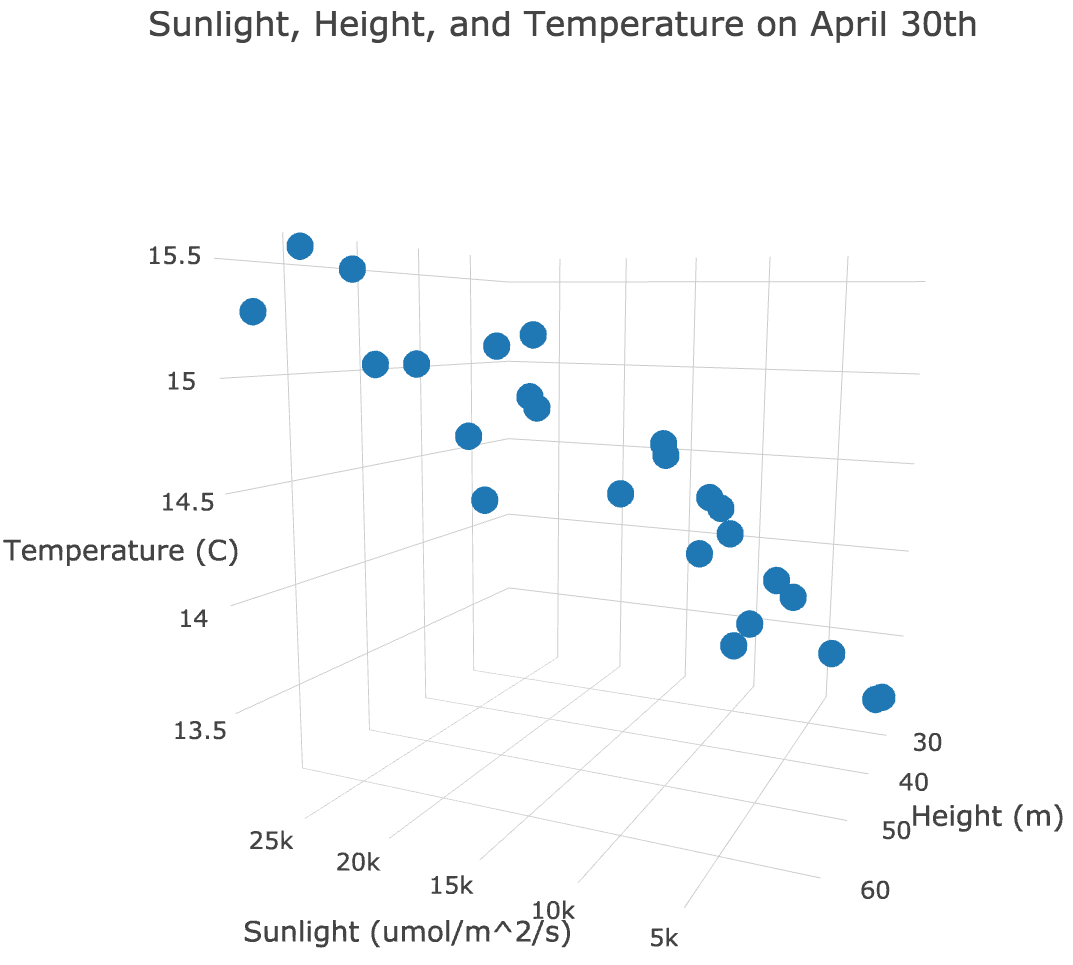
\includegraphics[scale=.75]{plot3.png}
\end{center}

\begin{knitrout}
\definecolor{shadecolor}{rgb}{0.969, 0.969, 0.969}\color{fgcolor}
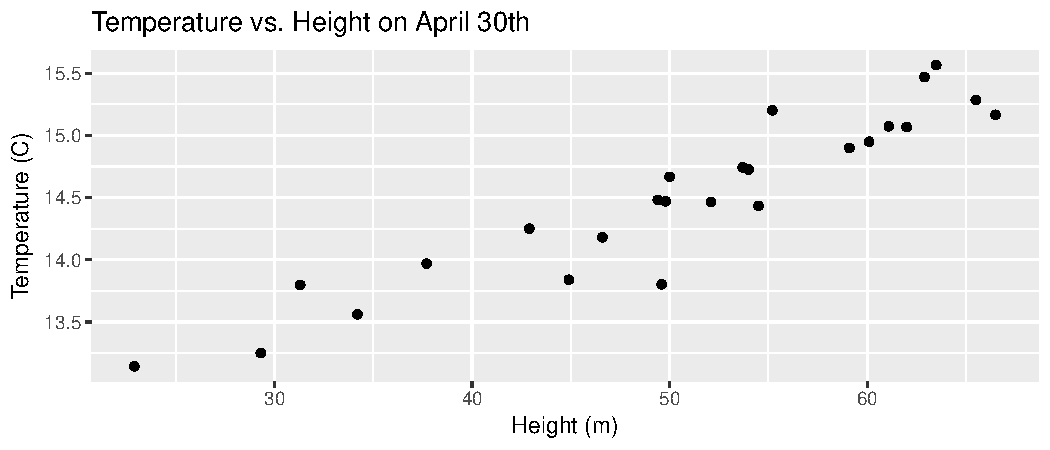
\includegraphics[width=\maxwidth]{figure/q3-1} 

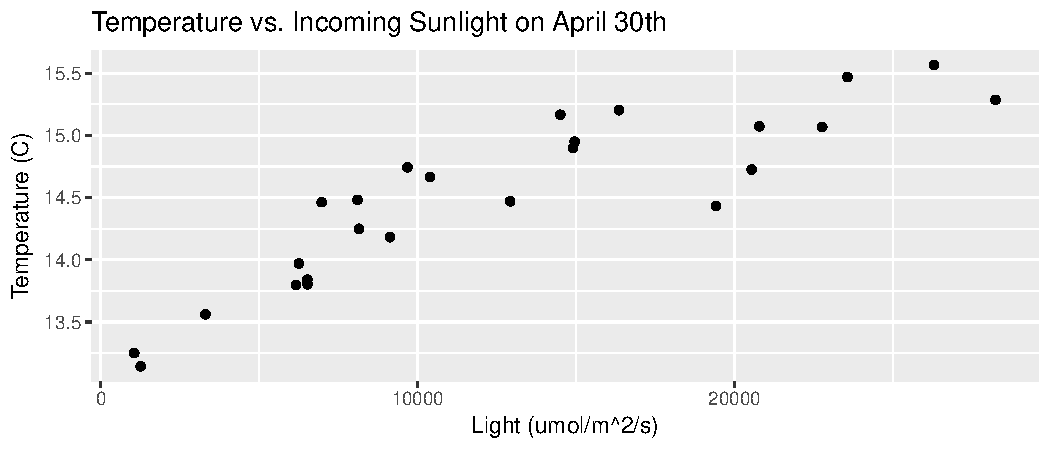
\includegraphics[width=\maxwidth]{figure/q3-2} 

\end{knitrout}

As we might expect, increased height and sunlight exposure correspond to higher temperatures.

\section{Discussion}

The data size was not challenging computationally, but it was necessary to subset the data by
days in order to show the trends and analyses clearly.  Further work could be done representing the 
month's worth of data effectively all at once.

\section{Conclusion}

This lab offered an opportunity to see how different data cleaning 
methodologies alter the conclusions of an experiment.  It allows showed how 
choices of which data to use can vary between question to question of the 
data set.  Through the redwood meteorlogical and sunlight information, we 
are able to establish interesting physical relationships that resonate well
with our understanding of basic physical and biological principles.

\section{Acknowledgements}

The author gratefully thanks Max Andrew Gardner, a fellow student in this course, for assistance with the lab.

\end{document}
